%% LaTeX-Beamer template for KIT design
%% by Erik Burger, Christian Hammer
%% title picture by Klaus Krogmann
%%
%% version 2.0
%%
%% mostly compatible to KIT corporate design v2.0
%% http://intranet.kit.edu/gestaltungsrichtlinien.php
%%
%% Problems, bugs and comments to
%% burger@kit.edu

\documentclass[18pt]{beamer}
\usetheme{kit}

%% TITLE PICTURE

% if a custom picture is to be used on the title page, copy it into the 'logos'
% directory, in the line below, replace 'mypicture' with the 
% filename (without extension) and uncomment the following line
% (picture proportions: 63 : 20, *.eps format if you use latex+dvips+ps2pdf,
% *.jpg/*.png/*.pdf if you use pdflatex)

%\titleimage{mypicture}

%% TITLE LOGO

% for a custom logo on the front page, copy your file into the 'logos'
% directory, insert the filename in the line below and uncomment it

%\titlelogo{mylogo}

% (*.eps format if you use latex+dvips+ps2pdf,
% *.jpg/*.png/*.pdf if you use pdflatex)

%% BIBTEX ICON/KEY

% if you want to see BibTeX keys in the references view instead of the symbol,
% uncomment the following line
% \usebibitemtemplate{\insertbiblabel}

% the presentation starts here

% change the following line to "ngerman" for German style date and logos
% change the following line to "english" for English style date and logos
\selectlanguage{ngerman}

\beamertemplatenavigationsymbolsempty

\usepackage{listings}
\definecolor{darkgray}{rgb}{0.95,0.95,0.95}
\definecolor{darkgreen}{rgb}{0.05,0.7,0.05}
\lstset{ language=Java,
	backgroundcolor=\color{darkgray}, 
	numbers=none, 
	keywordstyle=\color{black}\bfseries,
	tabsize=2,
	showspaces=false,               % show spaces adding particular underscores
	showstringspaces=false,         % underline spaces within strings
	showtabs=false, 
}



\title[Tutorium04]{Tutorium 04: Entwurfsmuster}
\subtitle{Softwaretechnik im SS 2011, Tutorium 4}
\author{Jürgen Walter}
\date{\today}

\institute{Chair for Software Design and Quality}

\begin{document}

%title page
\begin{frame}
\titlepage
\end{frame}

%table of contents
\frame{
\frametitle{Was machen wir heute?}
	\tableofcontents
}

\section{Altes Übungsblatt}

\subsection{Altes Übungsblatt}
\frame {
\frametitle{Altes Übungsblatt}
	\begin{block}{Aufgabe 1 - UML Zustandautomaten}
	\begin{itemize}
	\item ???
	\end{itemize}
	\end{block}
}


\begin{frame}[fragile]
\frametitle{Altes Übungsblatt}
	\begin{block}{Aufgabe 2 - Überladen und Überschreiben}
	\begin{itemize}
	\item ???
	\end{itemize}
	\end{block}
	\pause
	\begin{block}{Aufgabe 3 - JMJRST erweitern} 
	\begin{itemize}
	\item ???
	\end{itemize}
	\end{block}
\end{frame}

\frame{
\frametitle{Altes Übungsblatt}
	\begin{block}{Bonusaufgabe - Kammerjäger}
	\begin{itemize}
	\item wer hat den Debugger benutzt?
	\item bla?
	\end{itemize}
	\end{block}
}

\subsection{Zum Aufwärmen ...}
\frame {
\frametitle{Wahr oder falsch?}
\begin{itemize}
	\color<2->[rgb]{1,0,0}
	\item Implementierungsvererbung ist die Voraussetzung für Signaturvererbung 
	\color[rgb]{0,0,0}
	\pause
	\color<3->[rgb]{0,1,0}
	\item Ein Modul ist eine Menge von Programmelementen, die nach dem Geheimnisprinzip gemeinsam entworfen und geändert werden.
	\color[rgb]{0,0,0}
	
	\pause
	\color<4->[rgb]{1,0,0}
	\item Wenn eine Benutzthierarchie nur transitive Zyklen aufweist, heißt sie Benutztrelation
	\color[rgb]{0,0,0}
	\pause
	\color<5->[rgb]{1,0,0}
	\item Software ist leichter zu ändern als ein physisches Produkt vergleichbarer Komplexität.
	\color[rgb]{0,0,0}
	\pause
	\color<6->[rgb]{1,0,0}
	\item In Java muss eine abstrakte Klasse, die eine Schnittstelle implementiert, alle in der Schnittstelle vorgegebenen Methoden implementieren
	\color[rgb]{0,0,0}

\pause
	\color<7->[rgb]{0,1,0}
	\item Unter welchen Umständen ein Objekt welche Botschaft entgegen nimmt, spezifiziert man in einem UML-Zustandsdiagramm
	\color[rgb]{0,0,0}

\pause
	\color<8->[rgb]{0,1,0}
	\item Solange sich ein Objekt in einem Zustand befindet, reagiert es im gleichen Kontext immer gleich auf seine Umwelt
	\color[rgb]{0,0,0}
\end{itemize}
}

\frame {
\frametitle {Klausuraufgaben zum Aufwärmen} 
	\begin{block} {Aufgabe 1 (2P)}
	Nennen Sie 4 aus der Vorlesung bekannte Techniken zur Anforderungsermittlung während der 			
	Planungsphase. \\
	\visible<2-> {
	\begin{itemize}
		\item Fragebögen (engl. questionnaires)
		\item Interviews
		\item Aufgaben-
		\item Dokumenten-
		\item Systemanalyse
		\item Szenarien (engl. scenarios)
		\item Anwendungsfälle (engl. use cases)
	\end{itemize}
	}
	\end{block}
}

\frame {
\frametitle {Klausuraufgaben zum Aufwärmen} 
	\begin{block} {Aufgabe 2 (1,5P)}
	Nennen Sie 3 Ergebnisartefakte der Planungsphase.\\
	\visible<2-> {
	\begin{itemize}
		\item Durchführbarkeitsstudie
		\item Lastenheft
		\item Projektkalkulation
		\item Projektplan
	\end{itemize}
	}
	\end{block}
}

\frame {
\frametitle {Klausuraufgaben zum Aufwärmen} 
	\begin{block} {Aufgabe 3 (2P)}
	Für welche vier Eigenschaften steht der Begriff „ACID“-Prinzip?\\
	\visible<2-> {
	\begin{itemize}
		\item Atomicity
		\item Consistency
		\item Isolation
		\item Durability
	\end{itemize}
	}
	\end{block} 
}

\section{Polymorphie}
\frame {
\frametitle {Polymorphie} 
	\begin{block} {Polymorphie}
	\begin{itemize}
		\item Polymorphie bedeutet Vielgestaltigkeit
	\end{itemize}
	\end{block} 

	\begin{block} {dynamische Polymorphie}
	\begin{itemize}
		\item Verwendung von Vererbung
	\end{itemize}
	\end{block} 

	\begin{block} {statisch Polymorphie}
	\begin{itemize}
		\item Überladen von Methoden
	\end{itemize}
	\end{block} 
}


\subsection{Vererbung}


\frame {
\frametitle {Vererbung} 
	\begin{block} {Signaturvererbung}
	\begin{itemize}
		\item Oberklasse gibt an, welche Methoden implementiert werden sollen
		\item Java: Implementieren eines Interfaces mit implements
	\end{itemize}
	\end{block} 

	\begin{block} {Implementierungsvererbung}
	\begin{itemize}
		\item Oberklasse hat Methoden schon implementiert
		\item Methode kann überschrieben werden (@Override)
		\item Java: Erweitern einer Klasse mit extends
	\end{itemize}
	\end{block} 

	\begin{block} {Frage}
	\begin{itemize}
		\item Gibt es eine Einschränkungen für die Vererbung?
		\visible<2-> {
		\item Ja, das Substitutionsprinzip
		}
	\end{itemize}
	\end{block} 
}

\subsection{Überladen}
\frame {
\frametitle{Überladen}
	\begin{block}{Methoden überladen \dots}
	\begin{itemize}
	\item statische Polymorpie
	\item Methoden einer Klasse mit gleichen Namen, aber unterschiedlicher Signatur
	\item Hat nichts mit Vererbung zu tun!
	\item Bequem für den Benutzer
	\end{itemize}
	\end{block}
}


\section{UML}
\subsection{Zustandsdiagramm}

\frame{
\frametitle {Zustandsdiagramm (Wiederholung)} 
	\begin{itemize}
	\item Beschreibt mögliche Zustände eines Objekts sowie mögliche Zustandsübergänge
	\item Der Zustandsübergang (Transition) wird durch ein Ereignis ausgelöst
	\begin{center}
	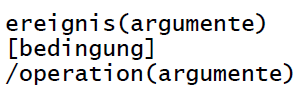
\includegraphics[scale=0.5]{pics/zustandsuebergang.png}
	\end{center}
	\item Zustandsübergang findet nur statt, wenn die Bedingung zu diesem Zeitpunkt erfüllt ist
	\item $\epsilon$ -Übergänge sind erlaubt
	\end{itemize}
}

\frame {
	\begin{exampleblock}{Zustandsdiagramm mit Gedächtnis (Wiederholung)}
	\begin{center}
	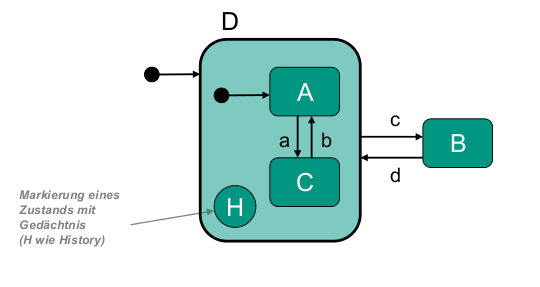
\includegraphics[scale=0.6]{pics/ZustandsDiagrammGedaechtnis.png}
	\end{center}
	\end{exampleblock}
}


\frame{
\frametitle {Klausuraufgabe 2009 (1P)}
	Gegeben ist der folgende UML-Zustandsautomat. Geben Sie an, in welcher Zustandskombination	
	sich der Zustandsautomat, jeweils ausgehend vom Startzustand, nach den beiden Eingabefolgen
	befindet. 
	\begin{itemize}
	\item Folge1: a, b, c, c   
	\visible<2-> {
	\item Zustandskombination: $A \times $D
	}
	\item Folge2: c, c, a, b, b, a, c, c, a
	\visible<3-> {
	\item Zustandskombination: $B \times $C
	}
	\end{itemize}
	\begin{center}
	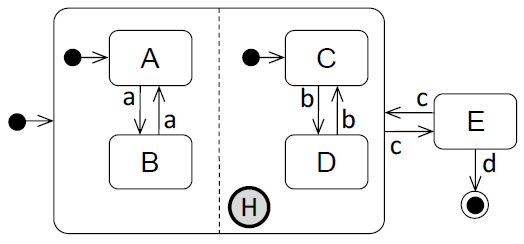
\includegraphics[scale=0.6]{pics/03/zustandN.png}
	\end{center}
}

\section{Ende}

\subsection{Tipps zum nächsten Übungsblatt}

\frame{
\frametitle{Tipps zum nächsten Übungsblatt}

	\begin{block}{Aufgabe 1 - Entwurfsmuster in der Java-API}
	\begin{itemize}
	\item Falls ihr nicht wisst, was die jeweiligen Code-Stellen tun, "googelt" euch Anwendungsbeispiele
	\item Stellt wirklich nur das allernotwendigste mit UML dar, denn diese Klassen sind recht groß
	\end{itemize}
	\end{block}

	\begin{block}{Aufgabe 2 - Kreuzworträtsel}
	\begin{itemize} \pause
	\item das sollte jeder mit den Entwurfsmustern aus der Vorlesung hinbekommen
	\item achtet darauf, den jeweiligen Namen aus der Vorlesung zu benutzen!
	\end{itemize}
	\end{block}
}


\frame{
\frametitle{Tipps zum nächsten Übungsblatt}
	\begin{block}{Aufgabe 3 - Entwurfsmuster anwenden}
	\begin{itemize}
	\item in beiden Projekten soll genau ein passendes Entwurfsmuster umgesetzt werden, um das Programm einfacher bzw. einfacher erweiterbar zu machen
	\item Abgabe besteht jeweils aus zwei Teilen:

		\begin{itemize}
		\item je ein Klassendiagramm auf Papier
		\item je ein Zip-Archiv mit dem umgebauten Programmcode
		\end{itemize}

	\end{itemize}
	\end{block}
}


\frame{
\frametitle{Bis zum nächsten Mal}
	\begin{center}
	
\includegraphics[height=200pt]{pics/04/04_comic}
	\end{center}
}

\end{document}
